%%%%%%%%%%%%%%%%%%%%%%%%%%%%%%%%%%%%%%%%%%%%%%%%%%%%%%%%%%%%%%%%%%%%%
%% This is a (brief) model paper using the achemso class
%% The document class accepts keyval options, which should include
%% the target journal and optionally the manuscript type. 
%%%%%%%%%%%%%%%%%%%%%%%%%%%%%%%%%%%%%%%%%%%%%%%%%%%%%%%%%%%%%%%%%%%%%
\documentclass[journal=jacsat,manuscript=article]{achemso}
\SectionNumbersOn
\usepackage{tikz} %Format quantum circuits
\usetikzlibrary{quantikz2}%Format quantum circuits

\usepackage{multicol}
\usepackage{graphicx}% Include figure files
\usepackage{graphicx}% Include figure files
\usepackage{dcolumn}% Align table columns on decimal point
\usepackage{bm}% bold math
%\usepackage[mathlines]{lineno}% Enable numbering of text and display math
%\linenumbers\relax % Commence numbering lines
\usepackage{pgffor}
\usepackage[utf8]{inputenc}
\usepackage[T1]{fontenc}
\usepackage{mathptmx}
\usepackage{listings}
\lstset{language=Python}
\usepackage{rotating} % Rotating table
\usepackage{caption}
\usepackage{subcaption}

\usepackage{color}
\usepackage{dcolumn} % decimal align in tables
\usepackage{bm} % bold math
\usepackage{graphicx}
\usepackage{multirow} % for table cells to span rows
\usepackage{pifont} % for checkmarks
\usepackage{epsfig}
\usepackage{amsmath} % matrix
% \usepackage{subfigure}
\usepackage{float}
\usepackage{booktabs}
\usepackage{tabularx}
\usepackage{natbib}
\usepackage{gensymb}
\setlength{\paperwidth}{8.5in}
\setlength{\paperheight}{11.0in}
\usepackage{rotating}
\usepackage{threeparttable}
\usepackage{comment}
%for corrections
\usepackage[normalem]{ulem}
\usepackage{hyperref} % allows hyperlinking for references
%%%%%%%%%%%%%%%%%%%%%%%%%%%%%%%%%%%%%%%%%%%%%%%%%%%%%%%%%%%%%%%%%%%%%
%% Place any additional packages needed here.  Only include packages
%% which are essential, to avoid problems later. Do NOT use any
%% packages which require e-TeX (for example etoolbox): the e-TeX
%% extensions are not currently available on the ACS conversion
%% servers.
%%%%%%%%%%%%%%%%%%%%%%%%%%%%%%%%%%%%%%%%%%%%%%%%%%%%%%%%%%%%%%%%%%%%%
\usepackage[version=3]{mhchem} % Formula subscripts using \ce{}
\usepackage{xcolor}
\usepackage{amsmath,amssymb,amsthm}
\usepackage{mathtools,physics}
\usepackage{subcaption}
% \usepackage{titling}
%%%%%%%%%%%%%%%%%%%%%%%%%%%%%%%%%%%%%%%%%%%%%%%%%%%%%%%%%%%%%%%%%%%%%
%% If issues arise when submitting your manuscript, you may want to
%% un-comment the next line.  This provides information on the
%% version of every file you have used.
%%%%%%%%%%%%%%%%%%%%%%%%%%%%%%%%%%%%%%%%%%%%%%%%%%%%%%%%%%%%%%%%%%%%%
%%\listfiles

%%%%%%%%%%%%%%%%%%%%%%%%%%%%%%%%%%%%%%%%%%%%%%%%%%%%%%%%%%%%%%%%%%%%%
%% Place any additional macros here.  Please use \newcommand* where
%% possible, and avoid layout-changing macros (which are not used
%% when typesetting).
%%%%%%%%%%%%%%%%%%%%%%%%%%%%%%%%%%%%%%%%%%%%%%%%%%%%%%%%%%%%%%%%%%%%%
\newtheorem{theorem}{Theorem}[section]
\newtheorem{corollary}{Corollary}
\newtheorem{lemma}[theorem]{Lemma}
\newtheorem{proposition}{Proposition}
\newtheorem{conjecture}{Conjecture}
\newtheorem{definition}[theorem]{Definition}
\newtheorem{assumption}[theorem]{Assumption}
% \newtheorem{example}[theorem]{Example}
\newtheorem{example}{Example}[section]
\newtheorem{remark}{Remark}

% Add line numbers, as requested by Nature
\usepackage{lineno}
% \linenumbers


\newcommand*\mycommand[1]{\texttt{\emph{#1}}}
\newcommand{\noteg}[1]{\textcolor{red}{({Grier: #1})}}
\newcommand{\notek}[1]{\textcolor{darkspringgreen}{({Kostas: #1})}}

\def\myvdots{\ \vdots\ }
%%%% HELPER CODE FOR DEALING WITH EXTERNAL REFERENCES
% (from an answer by cyberSingularity at http://tex.stackexchange.com/a/69832/226)
%%%

\usepackage{xcite}

%%%%%%%%%%%%%%%%%%%%%%%%%%%%%%%%%%%%%%%%%%%%%%%%%%%%%%%%%%%%%%%%%%%%%%%%
%----Helper code for dealing with external references----
% (by cyberSingularity at http://tex.stackexchange.com/a/69832/226)

\usepackage{xr}
\makeatletter

\newcommand*{\addFileDependency}[1]{% argument=file name and extension
\typeout{(#1)}% latexmk will find this if $recorder=0
% however, in that case, it will ignore #1 if it is a .aux or 
% .pdf file etc and it exists! If it doesn't exist, it will appear 
% in the list of dependents regardless)
%
% Write the following if you want it to appear in \listfiles 
% --- although not really necessary and latexmk doesn't use this
%
\@addtofilelist{#1}
%
% latexmk will find this message if #1 doesn't exist (yet)
\IfFileExists{#1}{}{\typeout{No file #1.}}
}\makeatother

\newcommand*{\myexternaldocument}[1]{%
\externaldocument{#1}%
\addFileDependency{#1.tex}%
\addFileDependency{#1.aux}%
}
%------------End of helper code--------------

% put all the external documents here!
\myexternaldocument{SI}
\newcommand{\siref}[1]{\ref{#1}}
%%%%%%%%%%%%%%%%%%%%%%%%%%%%%%%%%%%%%%%%%%%%%%%%%%%%%%%%%%%%%%%%%%%%%%%%


%%%%%%%%%%%%%%%%%%%%%%%%%%%%%%%%%%%%%%%%%%%%%%%%%%%%%%%%%%%%%%%%%%%%%
%% The document title should be given as usual. Some journals require
%% a running title from the author: this should be supplied as an
%% optional argument to \title.
%%%%%%%%%%%%%%%%%%%%%%%%%%%%%%%%%%%%%%%%%%%%%%%%%%%%%%%%%%%%%%%%%%%%%
\title{A Combinatorial Search of Parameterized Quantum Circuit Learning for Chemical Applications}
%%%%%%%%%%%%%%%%%%%%%%%%%%%%%%%%%%%%%%%%%%%%%%%%%%%%%%%%%%%%%%%%%%%%%
%% Meta-data block
%% ---------------
%% Each author should be given as a separate \author command.
%%
%% Corresponding authors should have an e-mail given after the author
%% name as an \email command. Phone and fax numbers can be given
%% using \phone and \fax, respectively; this information is optional.
%%
%% The affiliation of authors is given after the authors; each
%% \affiliation command applies to all preceding authors not already
%% assigned an affiliation.
%%
%% The affiliation takes an option argument for the short name.  This
%% will typically be something like "University of Somewhere".
%%
%% The \altaffiliation macro should be used for new address, etc.
%% On the other hand, \alsoaffiliation is used on a per author basis
%% when authors are associated with multiple institutions.
%%%%%%%%%%%%%%%%%%%%%%%%%%%%%%%%%%%%%%%%%%%%%%%%%%%%%%%%%%%%%%%%%%%%%
\author{Grier M. Jones}
\affiliation[UTSG ECE]{
The Edward S. Rogers Sr. Department of Electrical and Computer Engineering, 
University of Toronto, 
10 Kings College Road, Toronto, Ontario, 
Canada M5S 3G4}
\alsoaffiliation[UTM CHEM]{
Department of Chemical and Physical Sciences, 
University of Toronto Mississauga, 
3359 Mississauga Road, Mississauga, Ontario, 
Canada L5L 1C6}

\author{Nick Taylor}
\affiliation[UTSG ECE]{
The Edward S. Rogers Sr. Department of Electrical and Computer Engineering, 
University of Toronto, 
10 Kings College Road, Toronto, Ontario, 
Canada M5S 3G4}
          
\author{Viki Kumar Prasad}
\affiliation[UTSG ECE]{
The Edward S. Rogers Sr. Department of Electrical and Computer Engineering, 
University of Toronto, 
10 Kings College Road, Toronto, Ontario, 
Canada M5S 3G4}
\alsoaffiliation[UTM CHEM]{
Department of Chemical and Physical Sciences, 
University of Toronto Mississauga, 
3359 Mississauga Road, Mississauga, Ontario, 
Canada L5L 1C6}



\author{Ulrich Fekl}
\affiliation[UTM CHEM]{
Department of Chemical and Physical Sciences, 
University of Toronto Mississauga, 
3359 Mississauga Road, Mississauga, Ontario, 
Canada L5L 1C6}
\email{ulrich.fekl@utoronto.ca}

\author{Hans-Arno Jacobsen}
\affiliation[UTSG ECE]{
The Edward S. Rogers Sr. Department of Electrical and Computer Engineering, 
University of Toronto, 
10 Kings College Road, Toronto, Ontario, 
Canada M5S 3G4}
\email{jacobsen@eecg.toronto.edu}
%%%%%%%%%%%%%%%%%%%%%%%%%%%%%%%%%%%%%%%%%%%%%%%%%%%%%%%%%%%%%%%%%%%%%
%% Some journals require a list of abbreviations or keywords to be
%% supplied. These should be set up here, and will be printed after
%% the title and author information, if needed.
%%%%%%%%%%%%%%%%%%%%%%%%%%%%%%%%%%%%%%%%%%%%%%%%%%%%%%%%%%%%%%%%%%%%%
\abbreviations{}
\keywords{American Chemical Society, \LaTeX}

%%%%%%%%%%%%%%%%%%%%%%%%%%%%%%%%%%%%%%%%%%%%%%%%%%%%%%%%%%%%%%%%%%%%%
%% The manuscript does not need to include \maketitle, which is
%% executed automatically.
%%%%%%%%%%%%%%%%%%%%%%%%%%%%%%%%%%%%%%%%%%%%%%%%%%%%%%%%%%%%%%%%%%%%%
\newcommand{\R}{\mathbb{R}}

\begin{document}

\section*{Abstract}
Within the quantum machine learning (QML) field, parameterized quantum circuits (PQCs), built using fixed and parameterized gates, offer a hybrid approach for complex machine learning tasks. While many potential use cases have been proposed, the exploration of relevant datasets for chemists is lacking. Our study seeks to understand the possible advantages and disadvantages of PQCs for two chemically relevant datasets: one based on the bond separation energies of 49 different classes of bonds, called the BSE49 dataset, and another consisting of water confirmations, where coupled-cluster singles and doubles (CCSD) wave functions are predicted using electronic structure theory data from lower-level methods using the data-driven coupled-cluster (DDCC) method. In our study, we examine a combinatorial space of 14 data encoding layers and 12 variational (ansatz) layers, for a combined total of 168 PQCs. To calibrate our PQCs, we utilize a dataset of noisy linear, quadratic, and sine functions to explore the effects of the circuit width and depth, the effects of the feature set size, and various error mitigation techniques. Following this step, we similarly examine our chemically relevant datasets. Our work highlights the difficulties in encoding classical molecular representations in a PQC for predicting bond separation energies and the aptitude for PQCs for predicting molecular wave functions. \par

\newpage
\begin{itemize}
	\item Abstract
	\item Introduction
	\item Methods
	\item Datasets
	\item Results and Discussion
	\begin{itemize}
		\item Function fitting 
		\begin{itemize}
			\item All (5 + 16 qubit)
			\item RUD + AL (5 + 16 qubit)
			\item Error mitigation on FakeQuebec
		\end{itemize}
		\item BSE
		\begin{itemize}
			\item All 5 qubit
			\item Truncated 16 qubit set (cost analysis 5 qubit)
			\item RUD + AL (5 + 16 qubit)
			\item Real device (without error mitigation and with whatever the best is from function fitting)
		\end{itemize}		
		\item DDCC (5 qubit only because classically it can be done with 5 features!)
		\begin{itemize}
			\item Truncated  5 qubit set (based on BSE 5 qubit cost analysis)
			\item RUD + AL (5 qubit)
			\item Real device (without error mitigation and with whatever the best is from function fitting)
		\end{itemize}				
	\end{itemize}
	\item Conclusion
\end{itemize}

\newpage
\setcounter{secnumdepth}{1}
\section{Introduction}
Within the field of chemistry, tools such as machine learning and quantum computing have become popular due to the promise of discoverying new molecules and materials.
Machine learning in chemistry has already become a broadly applicable tool for exploring chemical compound space\cite{ramakrishnan_quantum_2014,ramakrishnan_big_2015}, accelerating wave functions\cite{townsend_data-driven_2019,jones_chapter_2023}, and for applications, such as catalysis and drug discovery.\cite{behler_perspective_2016,goh_deep_2017,sanchez-lengeling_{i}nverse_2018,butler_machine_2018,janet_machine_2020}
[Sentence about quantum computing]
Another popular avenue, which combines quantum computing and machine learning, is quantum machine learning (QML).
QML utilizes quantum algorithms during some portion of the machine learning process in an attempt to outperform classical algorithms. \cite{biamonte_quantum_2017}
On the current era of quantum computers, parameterized quantum circuits (PQCs) offer an example of QML that is performed using a hybrid quantum-classical feedback loop, where the variational parameters are optimized classical, while the circuit is ran on quantum hardware.\cite{benedetti_parameterized_2019,suzuki_predicting_2020}

PQCs are often composed using two different subcircuits: the encoding layer, which is used to encode the features into the quantum circuit, and variational layers, which are composed of parameterized gates which can be optimized classical. 



PQCs are composed of data-encoding and variational subcircuits, which can be repeated multiple times.


While several examples exist for PQCs applied to chemical applications, they are largely relegated to drug discovery\cite{suzuki_predicting_2020,smaldone_quantum--classical_2024,ishiyama_noise-robust_2022,ranga_quantum_2024,alam_qnet_2022,avramouli_quantum_2023,avramouli_unlocking_2023,bhatia_quantum_2023} and experimental properties\cite{hatakeyama-sato_quantum_2023}.
Herein, we explore two different chemical datasets: one consisting of bond separation energies of 49 unique bond types, called the BSE49 dataset\cite{prasad_bse49_2021}, and another which utilizes data-driven coupled cluster (DDCC)\cite{townsend_data-driven_2019} to predict the coupled-cluster singles and doubles wave function parameters using lower-level quantum chemistry methods.

In this study, we create a robust Python code base for exploring a set of 14 data-encoding and 12 variational (ansatz) subcircuits for a total of 168 combined PQCs.
Our work includes the single and double encoding layers found in the paper of Suzuki and Katouda\cite{suzuki_predicting_2020}, including the encoding of Mitarai \textit{et al.}\cite{mitarai_quantum_2018}, along with using instantanious quantum polynomial (IQP) as an encoding layer. \cite{bremner_average-case_2015}
All of our variational (ansatz) layers can be found in the study of Sim \textit{et al.}\cite{sim_expressibility_2019}, where the expressiblity and entanglement capability of these circuits is analyzed.
We also examine the effects of the number of re-upload and ansatz layers, the effects of feature set size, and various error mitigation techniques. 







\cite{krenn_artificial_2023}

QML\cite{biamonte_quantum_2017}:
\begin{itemize}
	\item ``Quantum machine learning software makes use of quantum algorithms as part of a larger implementation. By analysing the steps that quantum algorithms prescribe, it becomes clear that they have the potential to outperform classical algorithms for specific problems (that is, reduce the number of steps required). This potential is known as quantum speedup.''
	\item ``The notion of a quantum speedup depends on whether one takes a formal computer science perspective—which demands mathematical proofs—or a perspective based on what can be done with realistic, finitesize devices—which requires solid statistical evidence of a scaling advantage over some finite range of problem sizes. For the case of quantum machine learning, the best possible performance of classical algorithms is not always known.''
	\item DO WE SEE THIS: ``Determination of a scaling advantage contrasting quantum and classical machine learning would rely on the existence of a quantum computer and is called a ‘benchmarking’ problem. Such advantages could include improved classification accuracy and sampling of classically inaccessible systems. Accordingly, quantum speedups in machine learning are currently characterized using idealized measures from complexity theory: query complexity and gate complexity (see Box 1 and Box 1 Table). Query complexity measures the number of queries to the information source for the classical or quantum algorithm. A quantum speedup results if the number of queries needed to solve a problem is lower for the quantum algorithm than for the classical algorithm. To determine the gate complexity, the number of elementary quantum operations (or gates) required to obtain the desired result are counted.''
	\item Input problem: ``Classical data must be input before being processed on a quantum computer. This ‘input problem’ often has little overhead but can present a serious bottleneck for certain algorithms. Likewise, the ‘output problem’ is faced when reading out data after being processed on a quantum device. Like the input problem, the output problem often causes a noticeable operational slowdown.''
	\item  QML challenges: ``These hardware challenges are technical in nature, and clear paths exist towards overcoming them. They must be overcome, however, if quantum machine learning is to become a ‘killer app’ for quantum computers. As noted previously, most of the quantum algorithms that have been identified face a number of caveats that limits their applicability. We can distill the caveats mentioned above into four fundamental problems. (1) The input problem. Although quantum algorithms can provide dramatic speedups for processing data, they seldom provide advantages in reading data. This means that the cost of reading in the input can in some cases dominate the cost of quantum algorithms. Understanding this factor is an ongoing challenge. (2) The output problem. Obtaining the full solution from some quantum algorithms as a string of bits requires learning an exponential number of bits. This makes some applications of quantum machine learning algorithms infeasible. This problem can potentially be sidestepped by learning only summary statistics for the solution state. (3) The costing problem. Closely related to the input/outputproblems, at present very little is known about the true number of gates required by quantum machine learning algorithms. Bounds on the complexity suggest that for sufficiently large problems they will offer huge advantages, but it is still unclear when that crossover point occurs. (4) The benchmarking problem. It is often difficult to assert that a quantum algorithm is ever better than all known classical machine algorithms in practice because this would require extensive benchmarking against modern heuristic methods. Establishing lower bounds for quantum machine learning would partially address this issue.''
\end{itemize}


PQCs\cite{benedetti_parameterized_2019}:
\begin{itemize}
	\item ``Parameterized quantum circuits (PQCs) offer a concrete way to implement algorithms and demonstrate quantum supremacy in the NISQ era. PQCs are typically composed of fixed gates, e.g. controlled NOTs, and adjustable gates, e.g. qubit rotations. Even at low circuit depth, some classes of PQCs are capable of generating highly non-trivial outputs. For example, under well-believed complexity-theoretic assumptions, the class of PQCs called instantaneous quantum polynomial-time cannot be efficiently simulated by classical resources (see Lund et al [3] and Harrow and Montanaro [4] for accessible Reviews of quantum supremacy proposals). The demonstration of quantum supremacy is an important milestone in the development of quantum computers. In practice, however, it is highly desirable to demonstrate a quantum advantage on applications. The main approach taken by the community consists in formalizing problems of interest as variational optimization problems and use hybrid systems of quantum and classical hardware to find approximate solutions. The intuition is that by implementing some subroutines on classical hardware, the requirement of quantum resources is significantly reduced, particularly the number of qubits, circuit depth, and coherence time. Therefore, in the hybrid algorithmic approach NISQ hardware focuses entirely on the classically intractable part of the problem.''
\end{itemize}

PQCs \cite{suzuki_predicting_2020}:
\begin{itemize}
	\item ``More recently, quantum machine learning (QML) [26–30] is a rapidly growing research field that combines near-term quantum algorithms and machine learning techniques. In particular, parameterized quantum circuits (PQCs) have been considered as machine learning models with high expressive power within the hybrid quantum–classical framework [31, 32]. PQCs are typically composed of fixed quantum gates (e.g., qubit rotations and entangling gates) in a shallow circuit layout, with variable parameters optimized in a classical feedback loop.''
	\item ``To our knowledge, however, the application of QML to regression tasks has not been fully investigated in the literature. It remains unclear what kinds of quantum states should be used in order to generate the feature map with high expressibility that is suited for real-world data sets.''
	\item ``quantitative structure–toxicity relationship (QSTR) models for predicting the toxicity of 221 phenols. While there are a variety of QSAR/QSTR models (e.g., 3D-QSAR [1, 4]),asafirst step we employ QSAR/QSTR models including molecular descriptors such as hydrophobicity, acidity constant, and frontier orbital energies. There have been quantum computations in biochemical and pharmaceutical areas, such as protein folding [43–45], molecular similarity [46], and biological data [47]; yet, there has been no study on quantum application to QSAR modeling, albeit an important part of ligand-based computer-aided drug design.''
	\item ``PQCs have been regarded as machine learning models with high expressive power within the framework of the hybrid quantum–classical approach. PQCs are usually composed of one-qubit rotations and two-qubit entangling operations in a shallow circuit layout, with parameters optimized in a feedback loop.''
	\item ``Combining near-term quantum algorithms and machine learning, QML using the framework of PQCs is sometimes referred to as quantum circuit learning (QCL)''
	\item ``PQCs consist of three components: the encoder circuit, the variational circuit, and the measurement for the estimation of the loss function''
	
\end{itemize}


PQCs \cite{hatakeyama-sato_quantum_2023}:
\begin{itemize}
	\item What they do: ``ntroduce quantum circuit learning (QCL) as an emerging regression algorithm for chemo- and materials-informatics. The supervised model, functioning on the rule of quantum mechanics, can process linear and smooth non-linear functions from small datasets (<100 records). Compared with conventional algorithms, such as random forest, support vector machine, and linear regressions, the QCL can offer better predictions with some one-dimensional functions and experimental chemical databases''
	\item ``Here, we introduce quantum circuit learning (QCL), an emerging algorithm for supervised learning.15–18 QCL works on the rule of quantum mechanics. It can predict various parameters likewise to classical models. The current quantum systems (noisy intermediate-scale quantum computers: NISQ)19,20 face the problems of calculation noise and the limited processable number of information units (qubits).''
	\item ``Since QCL is a frontier for machine learning, few reports have been published on authentic regression tasks. The success of prediction with a toxicity dataset of organic molecules was reported,17 whereas the study was still conceptual. The prediction processes and advantages have been unclear, especially from chemical and material viewpoints. Here, we conducted a more comprehensive study on QCL with standard datasets of one-dimensional functions and chemical properties. Both simulated and actual quantum computing was undertaken to clarify the challenges of QCL. Various hyperparameters were optimized for higher accuracy. The comparison with conventional models contrasted the benefits of the new approach: capable of learning both linear and non-linear functions even from small datasets. The property was also favorable for predicting the so-called extrapolating data region, which is essential for chemical and material research.''
	\item They cite \cite{takaki_learning_2021,suzuki_predicting_2020,mitarai_quantum_2018} as examples of PQCs/quantum circuit learning for regression task
	\item Justification for starting with 1D regression: ``Preliminary optimization of quantum circuits15,17 and our optimization revealed that the following configuration was concise and practical for regression tasks (for details, see results and explanations in Fig. S1''
\end{itemize}


\section{Methods}
PQCs are often constructed of three parts: encoding layers that are used to encode the features onto a quantum circuit, variational layers which include parameters that are optimized classically, and measurements which provide numerical estimations of the regression target values.\citep{suzuki_predicting_2020} 
In this study, we utilize the Mitarai (M)\cite{mitarai_quantum_2018}, single- (A1) and double-angle (A2) encoding layers found in Ref. \citep{suzuki_predicting_2020}, along with the instantaneous quantum polynomial (IQP) circuit found in Refs. \citep{bremner_average-case_2016} and \citep{havlicek_supervised_2019}.
In the following section, we follow the notations derived from  Ref. \citep{suzuki_predicting_2020}.
Encoding layers work mapping a $d$-dimensional feature vector, $\mathbf{x}=(x_{1}, x_{2}, \ldots, x_{d})^{T} \in \mathbb{R}^{d}$, normalized on the range $[-1,1]$, onto a quantum circuit using a unitary matrix, denoted as $U_{\Phi(\mathbf{x})}$, to produce the quantum state $U_{\Phi(\mathbf{x})}\ket{0}^{\otimes n}$, where $n$ are the number of qubits.
The encoding layer takes the following general form,
\begin{equation}
	U_{\Phi(x)} =  \prod_{l} E_{\text{ent}}^{l} U_{\phi_{l}(\mathbf{x})}
	\label{eq:general_encoding}
\end{equation}
where, $E_{\text{ent}}^{l}$ denotes the entangling gates, which can be a CNOT, CZ, or identity ($\mathbf{I}$) gates,   $U_{\phi_{l}(\mathbf{x})}$ denotes the choice of encoding unitaries. 
Like in  Ref. \citep{suzuki_predicting_2020}, we choose $l \in \{1, 2\}$, such that when $l=1$, $E_{\text{ent}}$ corresponds to an identity matrix and $U_{\Phi(x)} = U_{\phi_{1}(\mathbf{x})}$.

When $l=1$, $U_{\Phi(x)}$ can be one of the following four encoding layers: $U_{\text{A1}}$, $U_{\text{A2}}$, $U_{\text{M}}$, or $U_{\text{IQP}}$.
The single-angle encoding (Fig. \ref{fig:A1}) is the simplest and takes the following form,
\begin{equation}
	U_{\text{A1}} = \prod_{i=0}^{n} R^{Y}_{i}(x_{i}),
	\label{eq:A1}
\end{equation}
where $R^{Y}_{i}$ denotes a parameterized Y rotation gate on qubit $i$.
Like the single-angle encoding, the double-angle encoding (Fig. \ref{fig:A2}) utilizes a parameterized Y rotation gate on qubit $i$, with the addition of a parameterized Z rotation gate on qubit $i$, denoted as
\begin{equation}
	U_{\text{A2}} = \prod_{i=0}^{n}  R^{Z}_{i}(x_{i}) R^{Y}_{i}(x_{i}).
	\label{eq:A2}
\end{equation}
The Mitarai encoding layer (Fig. \ref{fig:M}) is a double-angle encoding layer with the addition of an arcosine function on the parameterized Z gate and arcsine on the parameterized Y gate,
\begin{equation}
	U_{\text{M}}  = \prod_{i=0}^{n} R^{Z}_{i}(\arccos (x_{i}^{2})) R^{Y}_{i}(\arcsin (x_{i}^{2})).
	\label{eq:M}
\end{equation}
Following the formulation provided in the PennyLane\cite{bergholm_pennylane_2022} software package, the IQP encoding layer (Fig. \ref{fig:IQP}) is defined as,
\begin{equation}
	U_{\text{IQP}}  = \prod_{i=0}^{n} H_{i} R^{Z}_{i}(x_{i})  \prod_{i<j} ZZ_{ij},
	\label{eq:IQP}
\end{equation}
where $H_{i}$ denotes a Hadamard gate on qubit $i$ and $ZZ_{ij}$ denotes a two-qubit entangline gate defined as $ZZ_{ij} = e^{-i x_{i} x_{j} \sigma_{z} \otimes \sigma_{z}}$.

  
  
\begin{figure}[H]
	\centering
	\begin{subfigure}{0.3\textwidth}
		\centering
		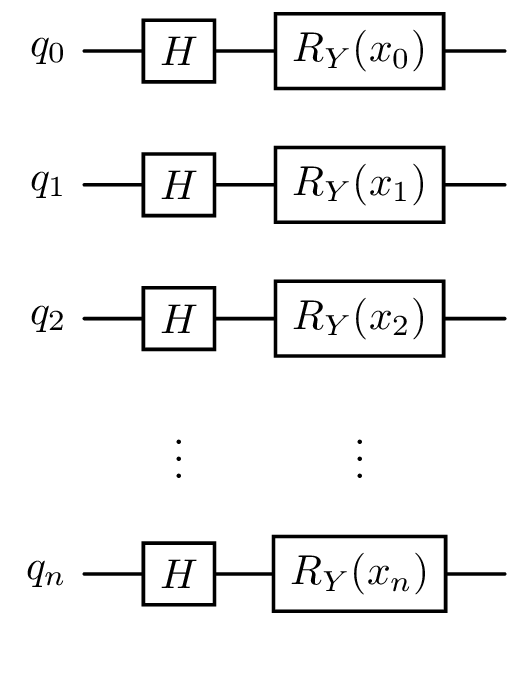
\includegraphics[width=\columnwidth]{images/encoders/quantikz/A1.png}
		\caption{}
		\label{fig:A1}		
	\end{subfigure}%
	\hfill
	\begin{subfigure}{0.3\textwidth}
		\centering
		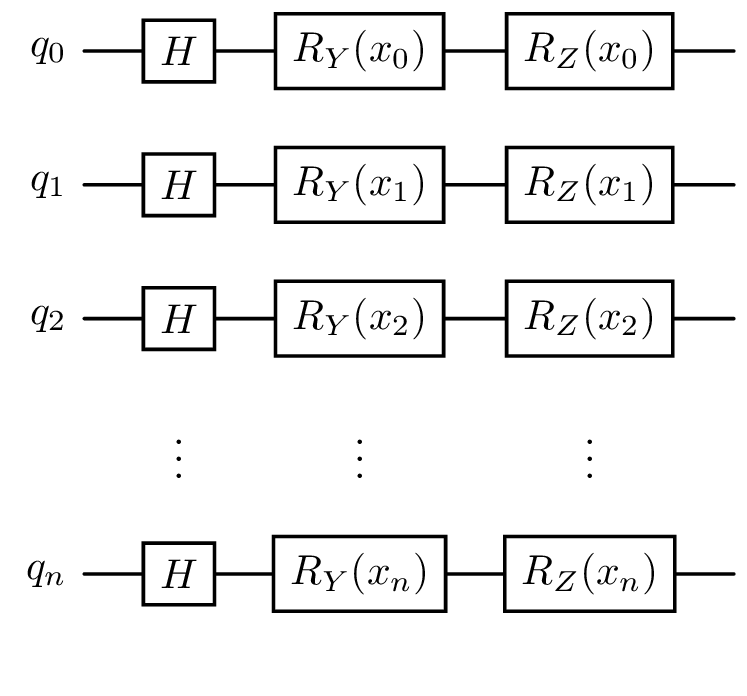
\includegraphics[width=\columnwidth]{images/encoders/quantikz/A2.png}
		\caption{}
		\label{fig:A2}		
	\end{subfigure}%
	\hfill
	\begin{subfigure}{0.3\textwidth}
		\centering
		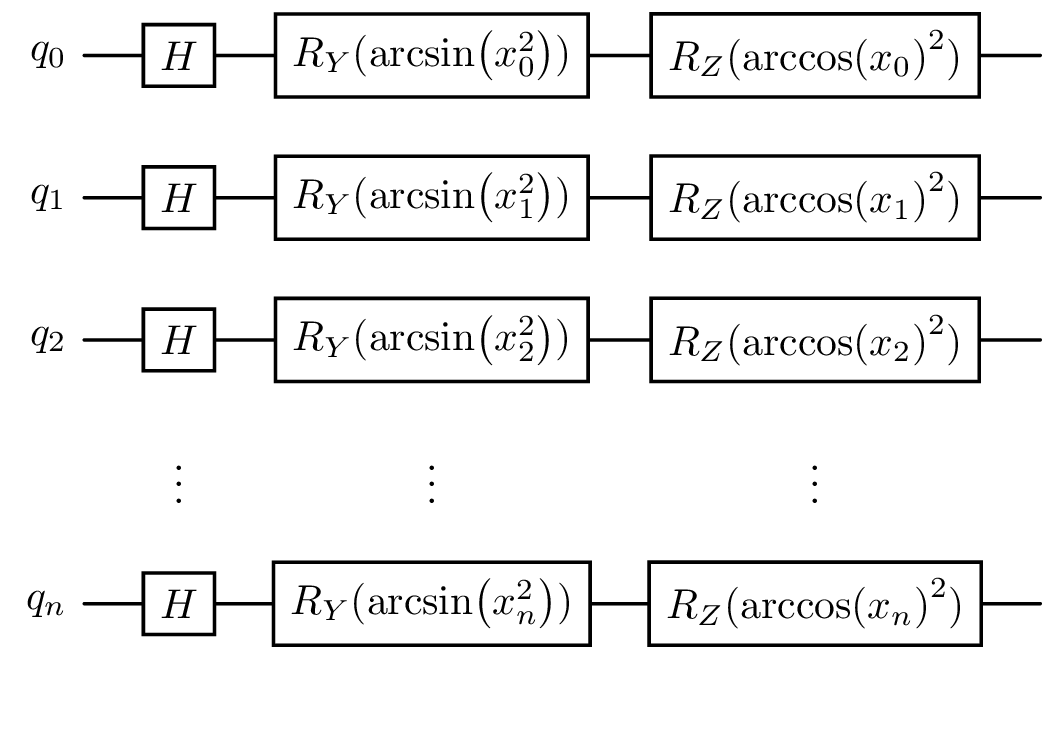
\includegraphics[width=1\columnwidth]{images/encoders/quantikz/M.png}
		\caption{}
		\label{fig:M}		
	\end{subfigure}%	  
	\hfill
	\begin{subfigure}{1\textwidth}
		\centering
		    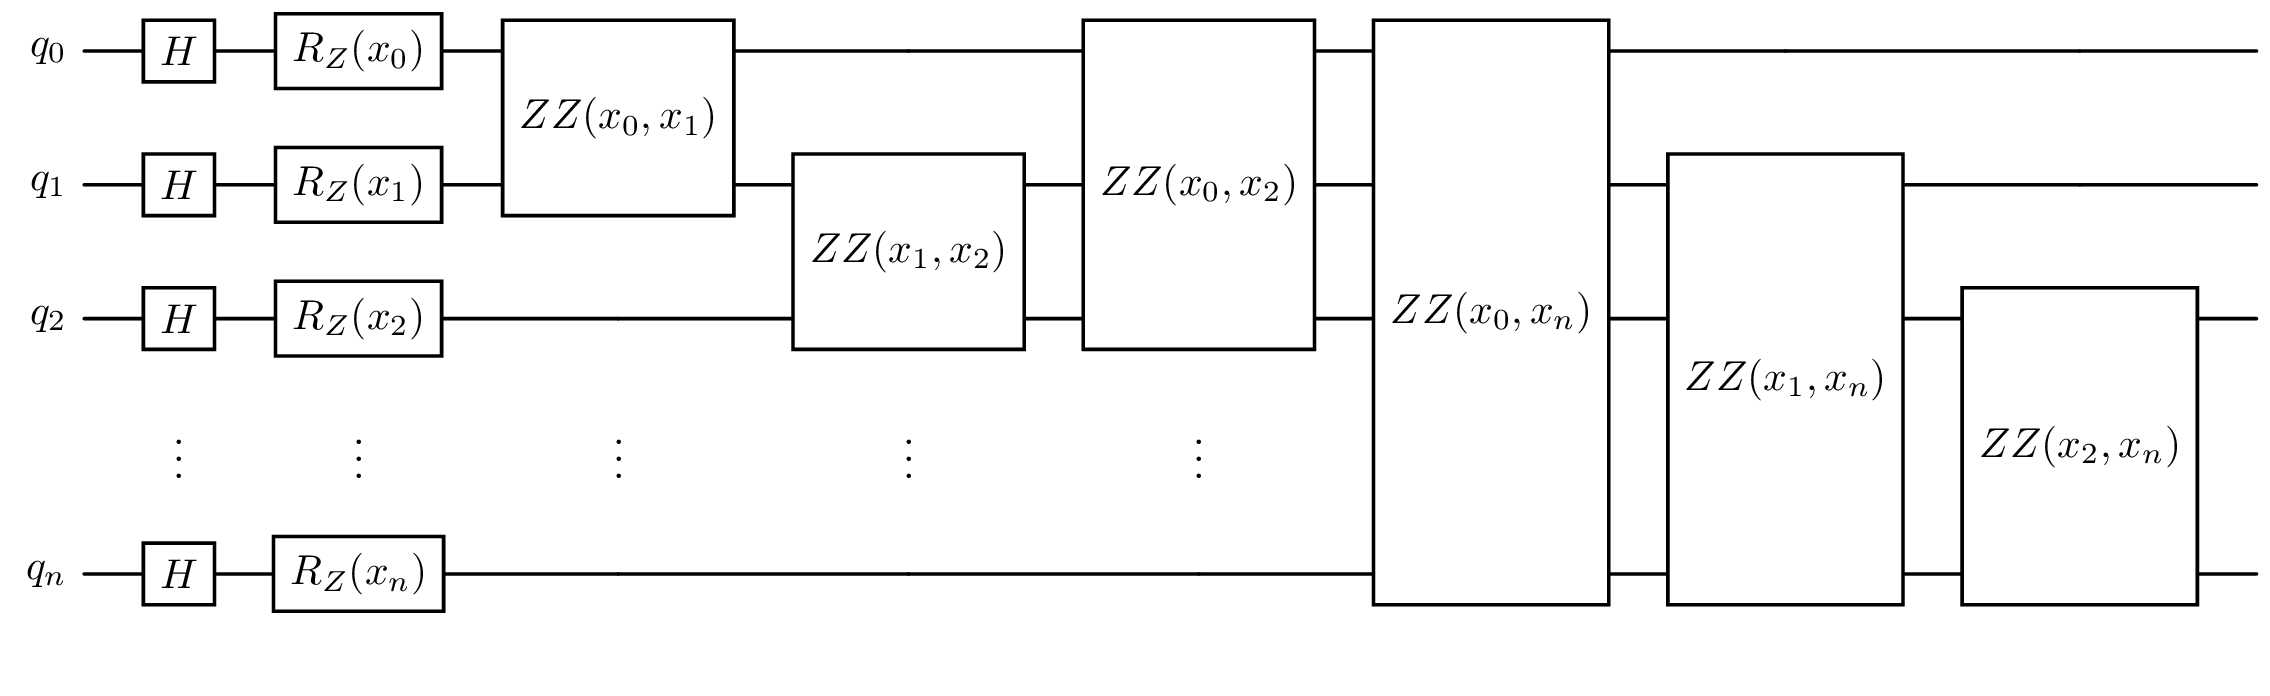
\includegraphics[width=\columnwidth]{images/encoders/quantikz/IQP.png}
		\caption{}
		\label{fig:IQP}
	\end{subfigure}%
	\caption{(a) Single angle (A1) encoding, (b) double angle (A2) encoding, (c) Mitarai (M) encoding, and (d) Instantaneous Quantum Polynomial (IQP) encoding}
	\label{fig:encoders}
\end{figure}





  
When $l=2$, like in Ref. \citep{suzuki_predicting_2020} we choose entanglement gates, $E_{\text{ent}}^{1}$ and $E_{\text{ent}}^{2}$ to be equivalent, and the encoding layer takes the following form, $U_{\Phi(x)} =  E_{\text{ent}} U_{\phi_{2}(\mathbf{x})} E_{\text{ent}} U_{\phi_{1}(\mathbf{x})}$ .
We also exclude IQP encoding when $l=2$ due to the increased circuit depth, when compared to A1, A2, and M encoding.
Therefore, there are five unique combinations of $U_{\phi_{1}(\mathbf{x})}$ and $U_{\phi_{2}(\mathbf{x})}$ (M-M, A1-A1, A2-A2, M-A1, and M-A2) and two different entanglement layer options (CNOT and CZ) for a total of 10 encoding circuits. 
These circuits are denoted as $U_{\phi_{1}(\mathbf{x})}-U_{\phi_{2}(\mathbf{x})}-E_{\text{ent}}$, for example, two example encoding circuits are M--M--CNOT and M--A1--CNOT.
Table \ref{tab:encoders} shows all fourteen encoding circuits examined in this study.

\begin{table}[htbp]
	\centering
	\begin{tabular}{|c|c|c|c|}
		\hline
		\textbf{Name} & $U_{\phi_{1}(\mathbf{x})}$ & $U_{\phi_{2}(\mathbf{x})}$ & $E_{\text{ent}}$  \\
		\hline
		\hline
		A1 & $U_{\text{A1}}$ & --- & --- \\
		\hline
		A2 & $U_{\text{A2}}$ & --- & --- \\
		\hline		
		M & $U_{\text{M}}$ & --- & --- \\
		\hline
		IQP & $U_{\text{IQP}}$ & --- & --- \\
		\hline
		A1--A1--CNOT & $U_{\text{A1}}$ & $U_{\text{A1}}$ & $E_{\text{CNOT}}$ \\
		\hline
		 A2--A2--CNOT & $U_{\text{A2}}$ & $U_{\text{A2}}$ & $E_{\text{CNOT}}$ \\
		\hline
		M--M--CNOT & $U_{\text{M}}$ & $U_{\text{M}}$ & $E_{\text{CNOT}}$ \\
		\hline
		M--A1--CNOT & $U_{\text{M}}$ & $U_{\text{A1}}$ & $E_{\text{CNOT}}$ \\
		\hline		
		M--A2--CNOT & $U_{\text{M}}$ & $U_{\text{A2}}$ & $E_{\text{CNOT}}$ \\
		\hline				
		A1--A1--CZ & $U_{\text{A1}}$ & $U_{\text{A1}}$ & $E_{\text{CZ}}$ \\
		\hline
		A2--A2--CZ& $U_{\text{A2}}$ & $U_{\text{A2}}$ & $E_{\text{CZ}}$ \\
		\hline
		M--M--CZ & $U_{\text{M}}$ & $U_{\text{M}}$ & $E_{\text{CZ}}$ \\
		\hline
		M--A1--CZ & $U_{\text{M}}$ & $U_{\text{A1}}$ & $E_{\text{CZ}}$ \\
		\hline		
		M--A2--CZ & $U_{\text{M}}$ & $U_{\text{A2}}$ & $E_{\text{CZ}}$ \\
		\hline						
	\end{tabular}
	\caption{Add something smart}
	\label{tab:encoders}
\end{table}



Following the encoding layers,variational (or ansatz) layers are used to introduce trainable parameters into the quantum circuit.
We use a mixed notation from Refs. \citep{suzuki_predicting_2020} and \citep{sim_expressibility_2019}, since Ref. \citep{sim_expressibility_2019} contains all of the variational layers used within this work.
We relegate the discussion of the expressibility and entanglement of these layers to Section \ref{section:results_and_discussion}


\begin{equation}
	U(\bm{\theta}) = \prod_{v} U_{v}(\bm{\theta}_{v}) E_{\text{ent}}^{v}
	\label{eq:general_variational}
\end{equation}



12 variational layers
ESU2
Efficient-CRX
Efficient-CRZ
Full-CRX
Full-CRZ
Full-Pauli-CRX
Full-Pauli-CRZ
HWE-CNOT
HWE-CZ
Hadamard
Modified-Pauli-CRX
Modified-Pauli-CRZ

\begin{quantikz}
	\lstick{$q_0$} & \gate{H} & \gate{R_{Y} (\arcsin(x_{0}^{2}))} & \gate{R_{Z} (\arccos(x_{0})^{2})} & \\
	\lstick{$q_1$} & \gate{H} & \gate{R_{Y} (\arcsin(x_{1}^{2}))} & \gate{R_{Z} (\arccos(x_{1})^{2})} & \\
	\lstick{$q_2$} & \gate{H} & \gate{R_{Y} (\arcsin(x_{2}^{2}))} & \gate{R_{Z} (\arccos(x_{2})^{2})} & \\
	\setwiretype{n} \lstick{}  & \myvdots & \myvdots & \myvdots & \\
	\lstick{$q_n$} & \gate{H} & \gate{R_{Y} (\arcsin(x_{n}^{2}))} & \gate{R_{Z} (\arccos(x_{n})^{2})} & \\
\end{quantikz}




\begin{equation}
	U(\bm{\theta}) U_{\Phi(\mathbf{x})}\ket{0}^{\otimes n} = \prod_{k}
	\left( \prod_{v} U_{v}(\bm{\theta}_{v}) E_{\text{ent}}^{v}   \prod_{l} E_{\text{ent}}^{l} U_{\phi_{l}(\mathbf{x})} \right)  \ket{0}^{\otimes n}
\end{equation}


$v \in \{1, 3, 5\}$
$k \in \{1, 3, 5\}$

\subsection{Implementation}
Our work was implemented in Python using PennyLane for constructing the quantum circuits, and Qulacs as a primary backend for simulating the circuits. The optimization was implemented using the scipy.optimize module from the SciPy library. Classical models were implemented using scikit-learn while processing of the data was handled with Pandas, NumPy, and SciPy libraries.  


Simulated using FakeQuebecbackend

\subsection{Dataset}
We trained our models using three datasets: a function fitting dataset, consisting of a noisy linear, quadratic, and sine function, used for model calibration; a dataset consisting of electronic structure features to predict wavefunctions using the data-driven coupled-cluster scheme of Townsend and Vogiatzis \cite{townsend_data-driven_2019}; and a dataset of bond separation energies (BSE) of molecules, where the feature set encodes structural information of each molecule. 

For the function fitting dataset, there is only one feature per target value.
For the DDCC dataset, there are initially X features, reduced down to 5 and 16 features, respectively, using SHapley Additive exPlanation (SHAP) values.\cite{lundberg_unified_2017} 


\begin{equation}
	t^{ab}_{ij(\text{MP2})} = \frac{\mel{ij}{}{ab}}{\varepsilon_{i}+\varepsilon_{j}-\varepsilon_{a}-\varepsilon_{b}}
	\label{eq:MP2_t2}
\end{equation}

For each $t^{ab}_{ij(\text{CCSD})}$, orbital energies ($\varepsilon_{i},\varepsilon_{j},\varepsilon_{a},\varepsilon_{b}$), Coulomb and exchange integrals ($J^{i}_{a},J^{j}_{b},K^{a}_{i},K^{b}_{j}$), binary feature whether two electrons are promoted to the same virtual orbital, the initial MP2 amplitudes, along with the numerator (two-electron integrals ($\mel{ij}{}{ab}$)) and denominator $\varepsilon_{i}+\varepsilon_{j}-\varepsilon_{a}-\varepsilon_{b}$.



For the BSE dataset, various molecular representations are explored, and we settled on using Morgan fingerprints with X parameters. 
For the feature reduction, we use PCA, as explained in Section



% Make distribution plot
%\begin{figure}[H]
%	\centering
%	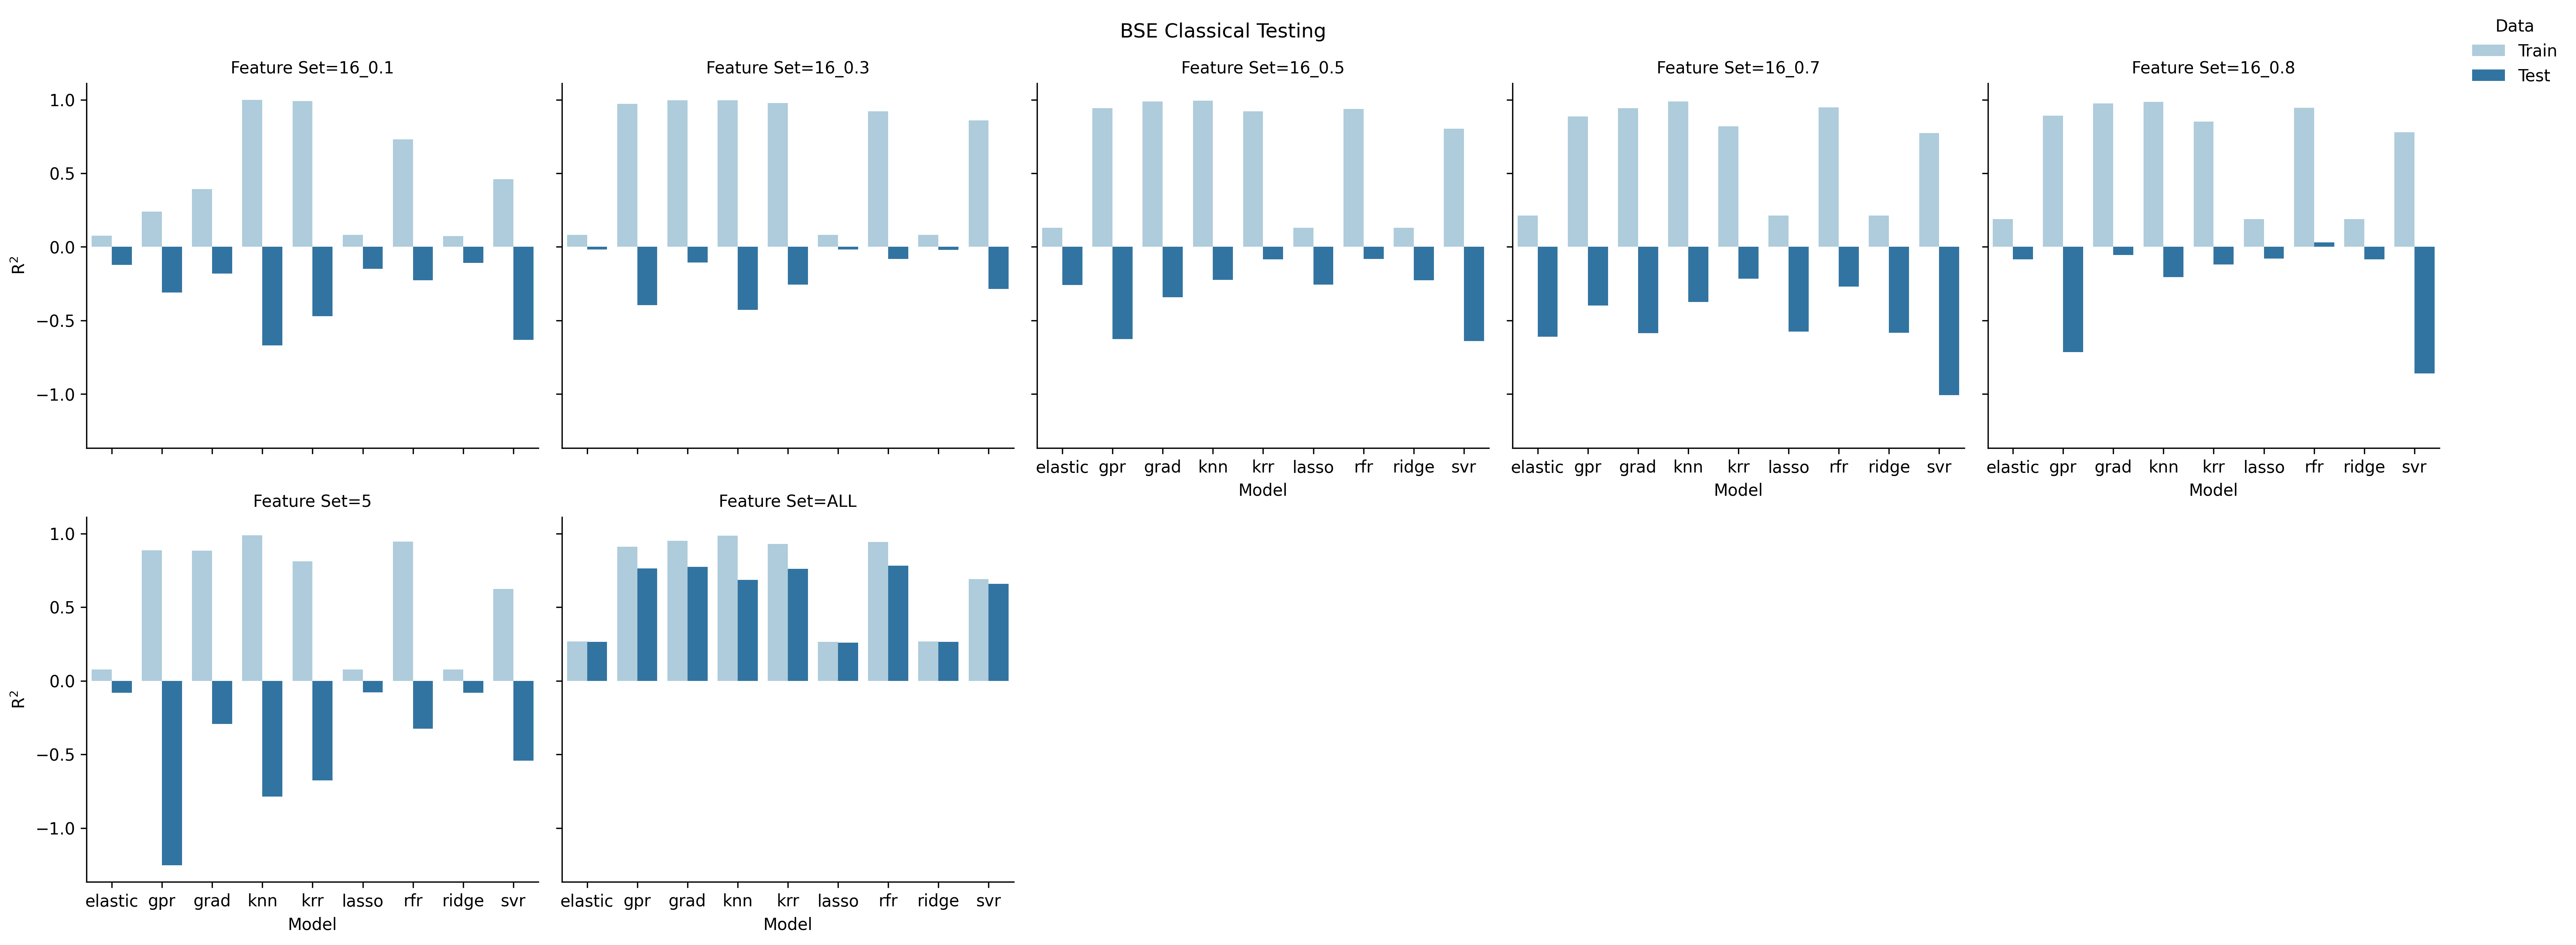
\includegraphics[width=\linewidth]{images/BSE.png}
%	\caption{BSE}
%	\label{fig:BSE}
%\end{figure}


\begin{figure}[H]
	\centering
	\begin{subfigure}[b]{0.3\textwidth}
		\centering
		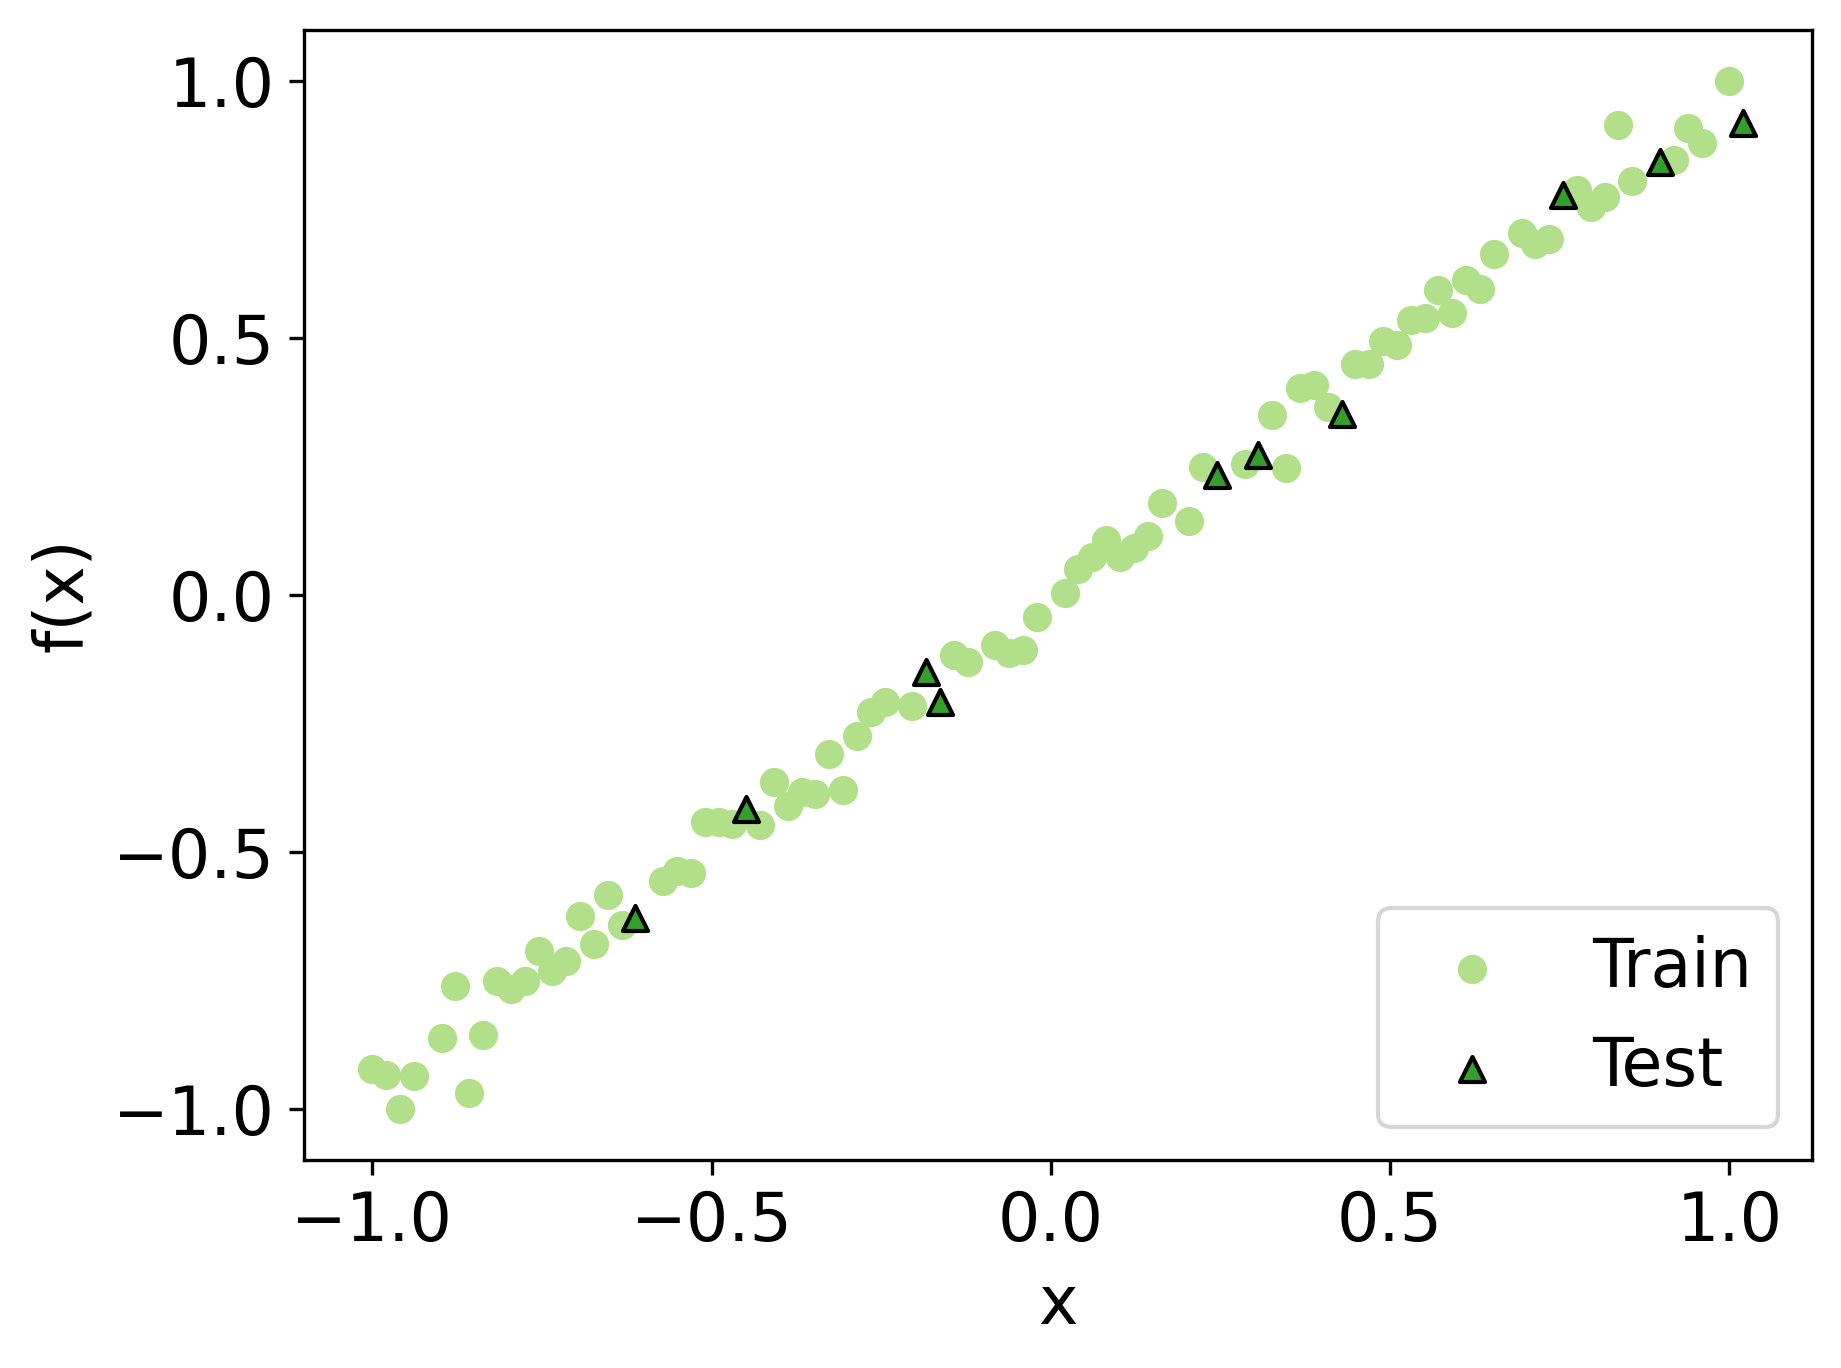
\includegraphics[width=\textwidth]{images/Function_Fitting/function_dataset/linear_train_vs_test.png}
		\caption{}
		\label{fig:linear_train_vs_test}
	\end{subfigure}
	\hfill
	\begin{subfigure}[b]{0.3\textwidth}
		\centering
		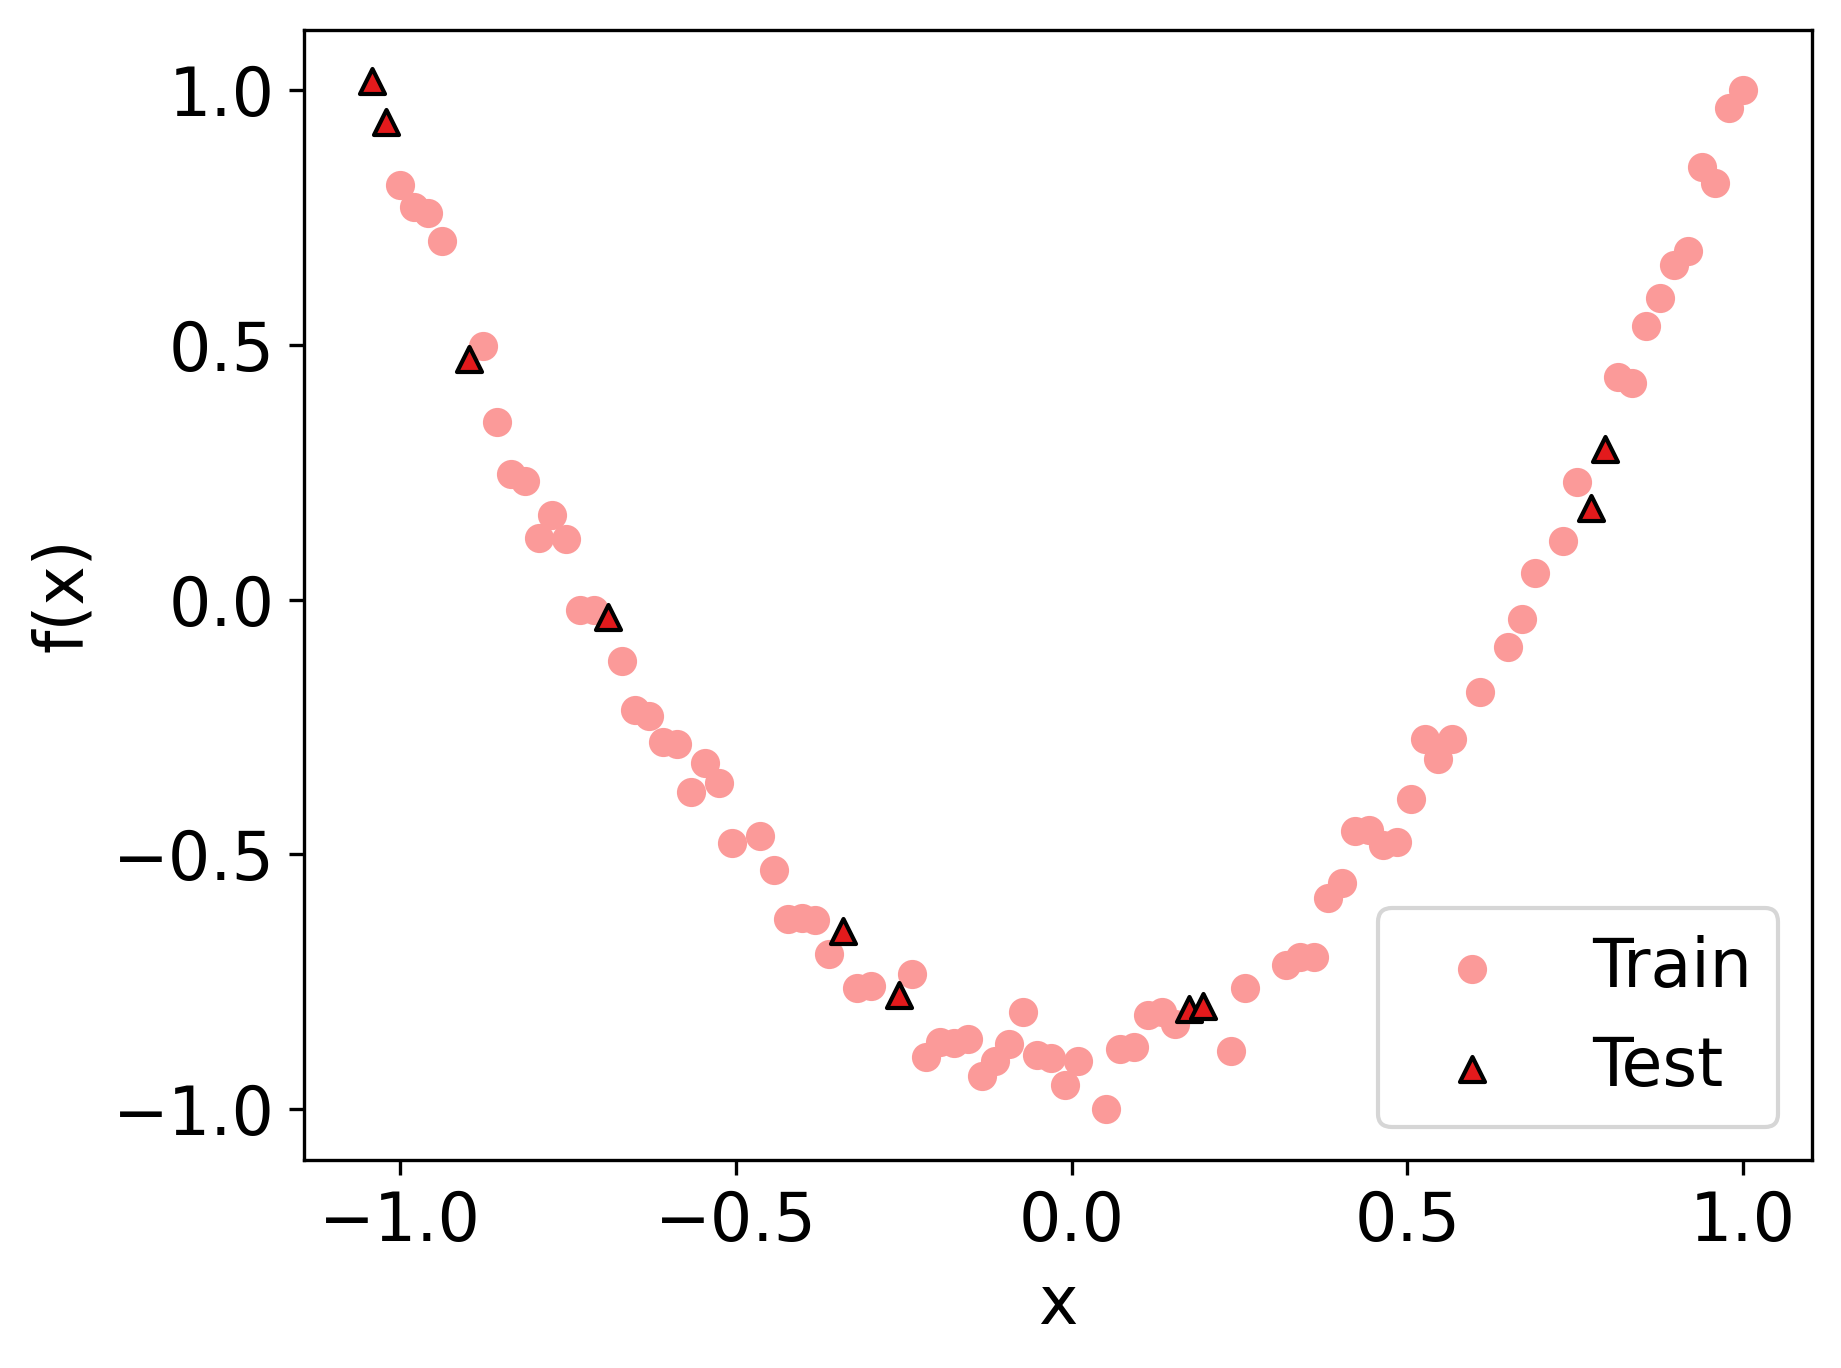
\includegraphics[width=\textwidth]{images/Function_Fitting/function_dataset/quadratic_train_vs_test.png}
		\caption{}
		\label{fig:quadratic_train_vs_test}
	\end{subfigure}
	\hfill
	\begin{subfigure}[b]{0.3\textwidth}
		\centering
		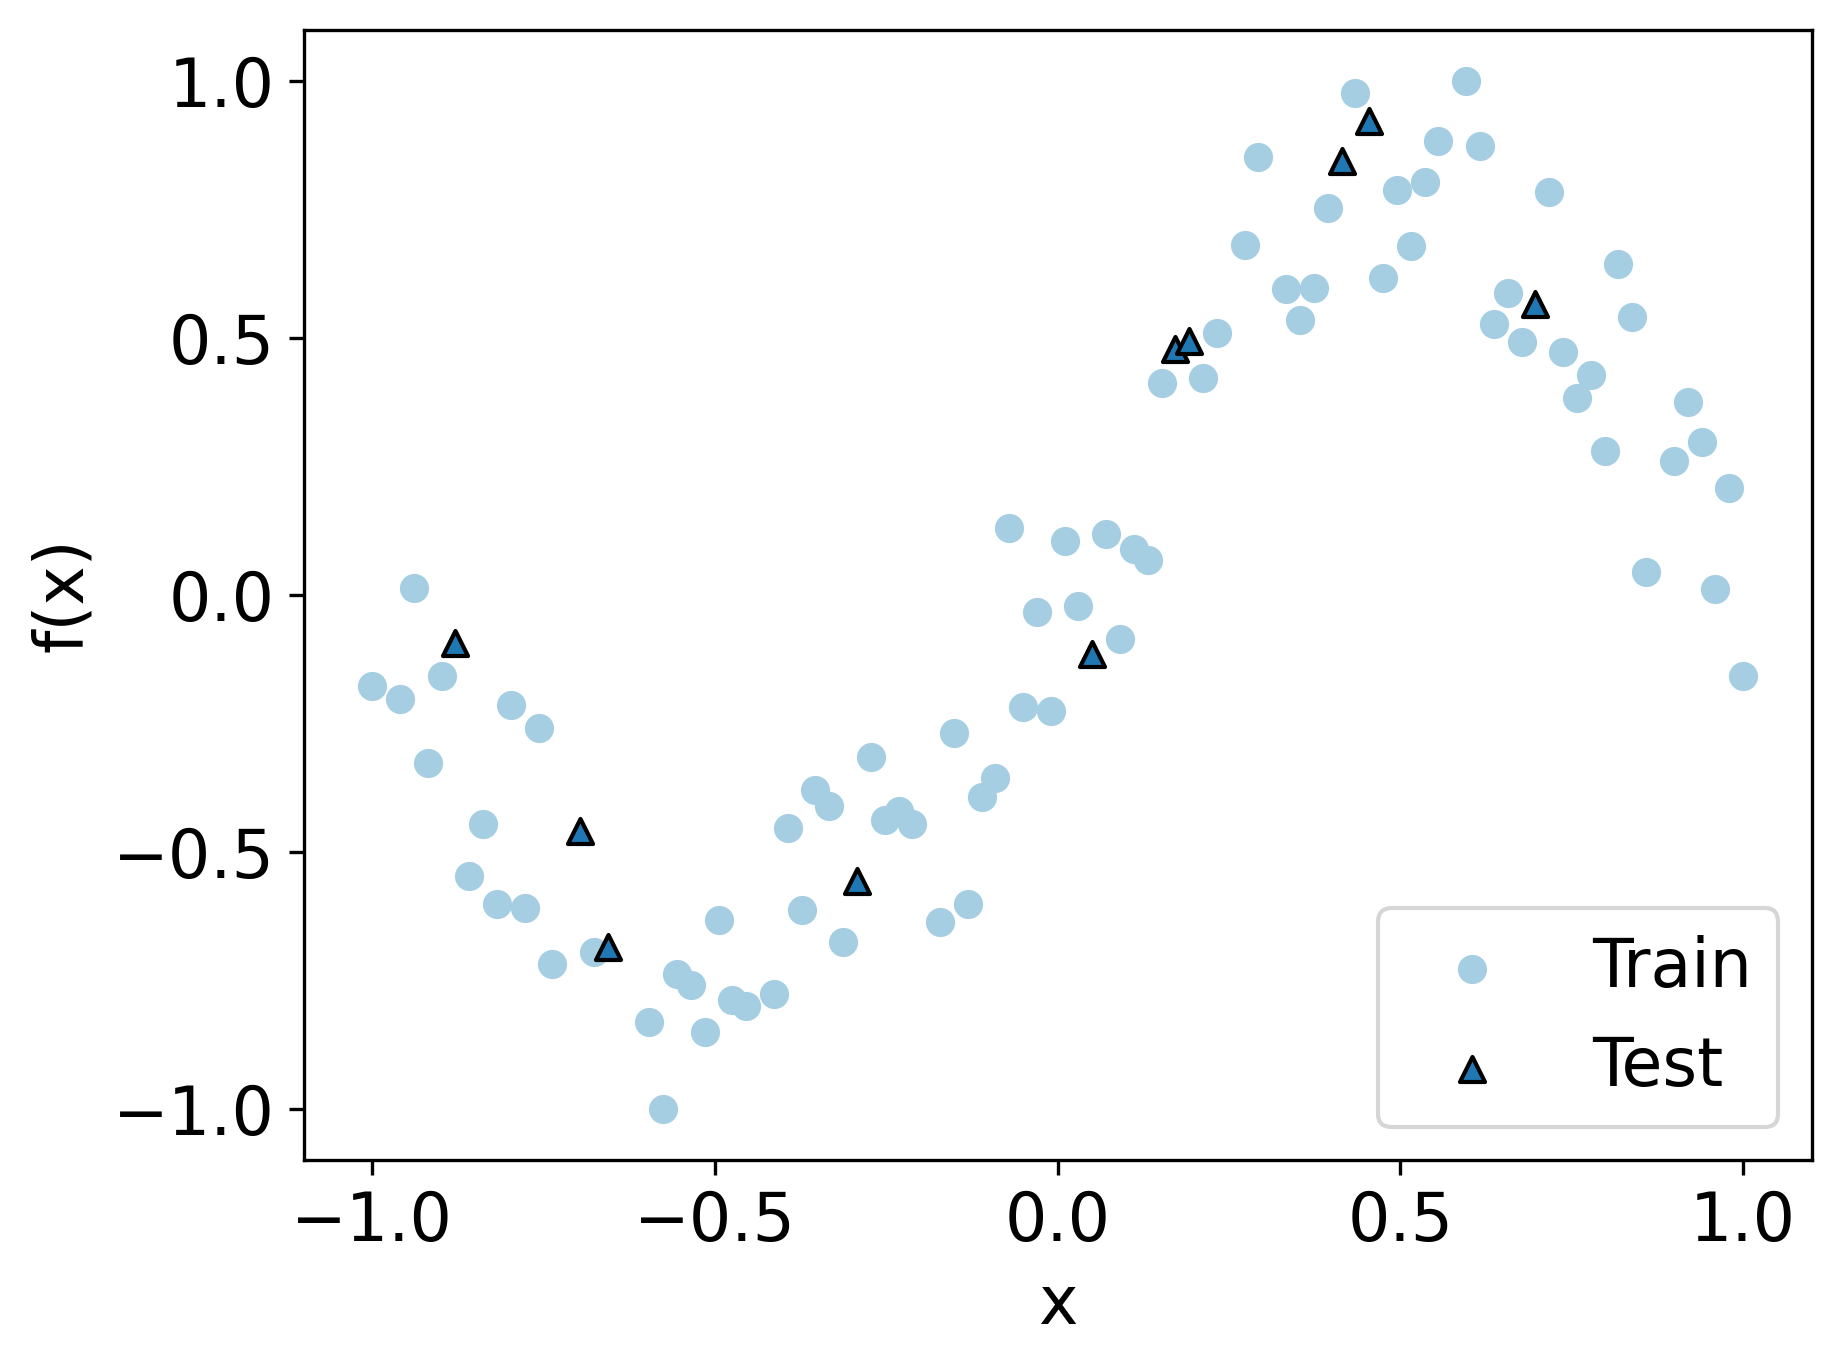
\includegraphics[width=\textwidth]{images/Function_Fitting/function_dataset/sine_train_vs_test.png}
		\caption{}
		\label{fig:sine_train_vs_test}
	\end{subfigure}
	\caption{}
	\label{fig:train_vs_test}
\end{figure}

\section{Results and Discussion}
\label{section:results_and_discussion}


Ansaetze analysis \cite{sim_expressibility_2019}
``In particular, a substantial improvement in performance of two-qubit gates in a ring or all-to-all connected arrangement, compared to thatof those on a line, is observed.''

``Furthermore, improvement in both descriptors is achieved by sequences of controlled X-rotation gates compared tosequences of controlled Z-rotation gates.''

``investigated howexpressibility “saturates” with increased circuit depth, finding that the rateand saturated value appear to be distinguishing features of a PQC''



\section{Conclusion}
Depth is not always better!
Molecular representations specifically for QML
Distributed QC to incorporate more features

\bibliography{achemso-demo}

\end{document}
